\section{CAD第五次作业}
\setcounter{subsection}{0}
\subsection{题目:}

\tt{题8计算获得电容值，置于A位置，仿真确认满足设计要求}

\tt{将电容从A位置移到B位置，仿真，说明是否满足设计要求}

\tt{将电容拆分为两个电容，分别置于A，B两个位置，…}

\tt{将电容拆分为3个电容，置于A，B及互导电阻中间，…}

\tt{将电容拆分为4个电容，置于A，B及互导、互阻电阻中间，…}

\tt{总结：功能电路的去耦电容应该置于什么位置最好？}

\tt{继续研究：模拟电路还是数字电路离电源更近了好？}

\begin{figure}[!ht]
\centering
\resizebox{1\textwidth}{!}{%
\begin{circuitikz}
\tikzstyle{every node}=[font=\normalsize]
\draw (3,11.25) to[american voltage source,l={ \normalsize 5V}] (3,8.5);
\draw (3,11.25) to[european resistor,l={ \normalsize $R_{1}=10\Omega$}] (6,11.25);
\draw (8.25,11.25) to[european resistor,l={ \normalsize $R_{2}=10\Omega$}] (11,11.25);
\draw (7.25,9.5) to[european resistor,l={ \normalsize $R_{a}=1k\Omega$}] (7.25,7);
\draw (12,7) to[european resistor,l={ \normalsize $R_{d1}=990\Omega$}] (12,9.25);
\draw (13.5,9.25) to[european resistor,l={ \normalsize $R_{d2}=90\Omega$}] (13.5,7);
\draw (6,11.25) to[short] (9,11.25);
\draw (10.25,11.25) to[short] (12.75,11.25);
\draw (12.75,11.25) to[short] (12.75,10);
\draw (12.75,10) to[short] (12.25,9.5);
\draw (3,8.5) to[short] (3,7);
\draw (3,7) to[short] (13.5,7);
\node [font=\normalsize] at (14.25,10.5) {开关频率10MHz};
\draw (7.25,11.25) to[short] (7.25,9.25);
\draw (3,7) to (3,6.25) node[ground]{};
\node [font=\normalsize] at (6.25,11.75) {A};
\node [font=\normalsize] at (11.75,11.75) {B};
\end{circuitikz}
}%
\caption{题目要求的电路图}
\label{fig:my_label}
\end{figure}

\subsection{A位置的电容:}

\tt{理论计算可得电容大小应为26.6nF}

\begin{figure}[!ht]
\centering
\resizebox{1\textwidth}{!}{%
\begin{circuitikz}
\tikzstyle{every node}=[font=\normalsize]
\draw (3,11.25) to[american voltage source,l={ \normalsize 5V}] (3,8.5);
\draw (3,11.25) to[european resistor,l={ \normalsize $R_{1}=10\Omega$}] (6,11.25);
\draw (8.25,11.25) to[european resistor,l={ \normalsize $R_{2}=10\Omega$}] (11,11.25);
\draw (7.25,9.5) to[european resistor,l={ \normalsize $R_{a}=1k\Omega$}] (7.25,7);
\draw (12,7) to[european resistor,l={ \normalsize $R_{d1}=990\Omega$}] (12,9.25);
\draw (13.5,9.25) to[european resistor,l={ \normalsize $R_{d2}=90\Omega$}] (13.5,7);
\draw (6,11.25) to[short] (9,11.25);
\draw (10.25,11.25) to[short] (12.75,11.25);
\draw (12.75,11.25) to[short] (12.75,10);
\draw (12.75,10) to[short] (12.25,9.5);
\draw (3,8.5) to[short] (3,7);
\draw (3,7) to[short] (13.5,7);
\node [font=\normalsize] at (14.25,10.5) {开关频率10MHz};
\draw (7.25,11.25) to[short] (7.25,9.25);
\draw (3,7) to (3,6.25) node[ground]{};
\node [font=\normalsize] at (6.25,11.75) {A};
\node [font=\normalsize] at (11.75,11.75) {B};
\draw (5.75,7) to[C,l={ \normalsize 26.6nF}] (5.75,9);
\draw (5.75,11.25) to[short] (5.75,8.75);
\end{circuitikz}
}%
\caption{A位置存在26.6nF电容的电路图}
\label{fig:my_label}
\end{figure}

\begin{figure}[H]
\centering
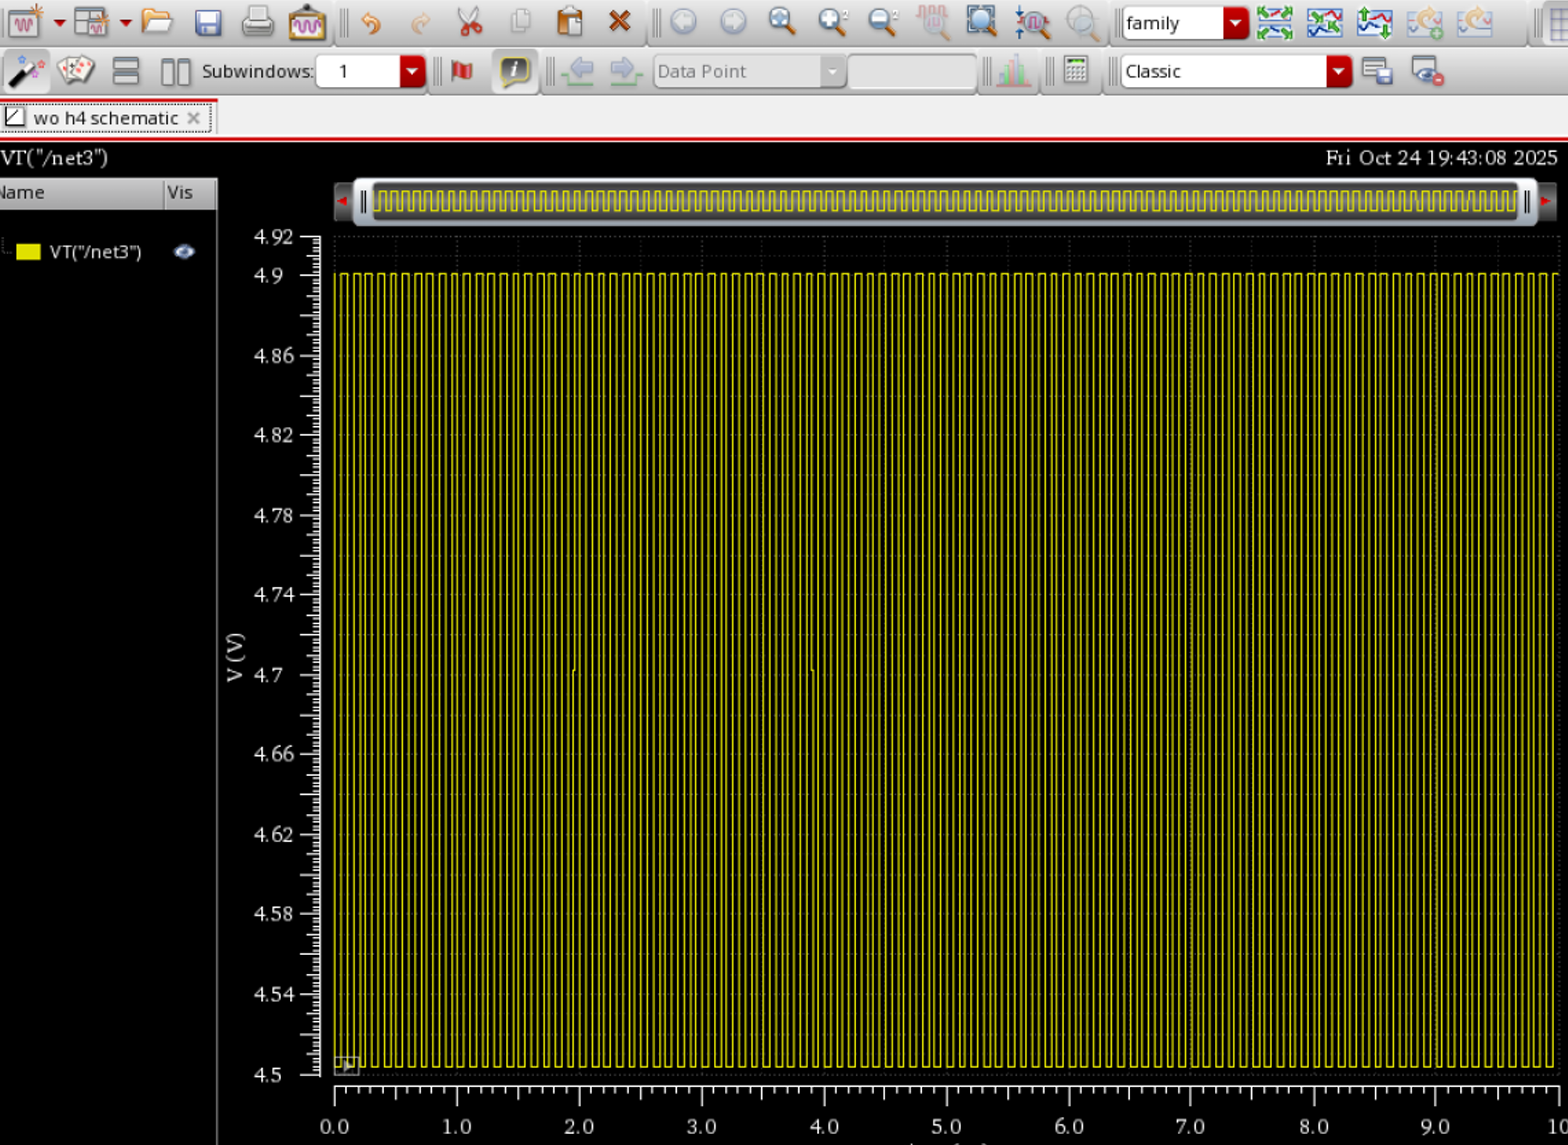
\includegraphics[width=0.8\textwidth]{chapters/figure/A20/无电容.png}
\caption{无电容结果}
\label{无电容结果}
\end{figure}

\begin{figure}[H]
\centering
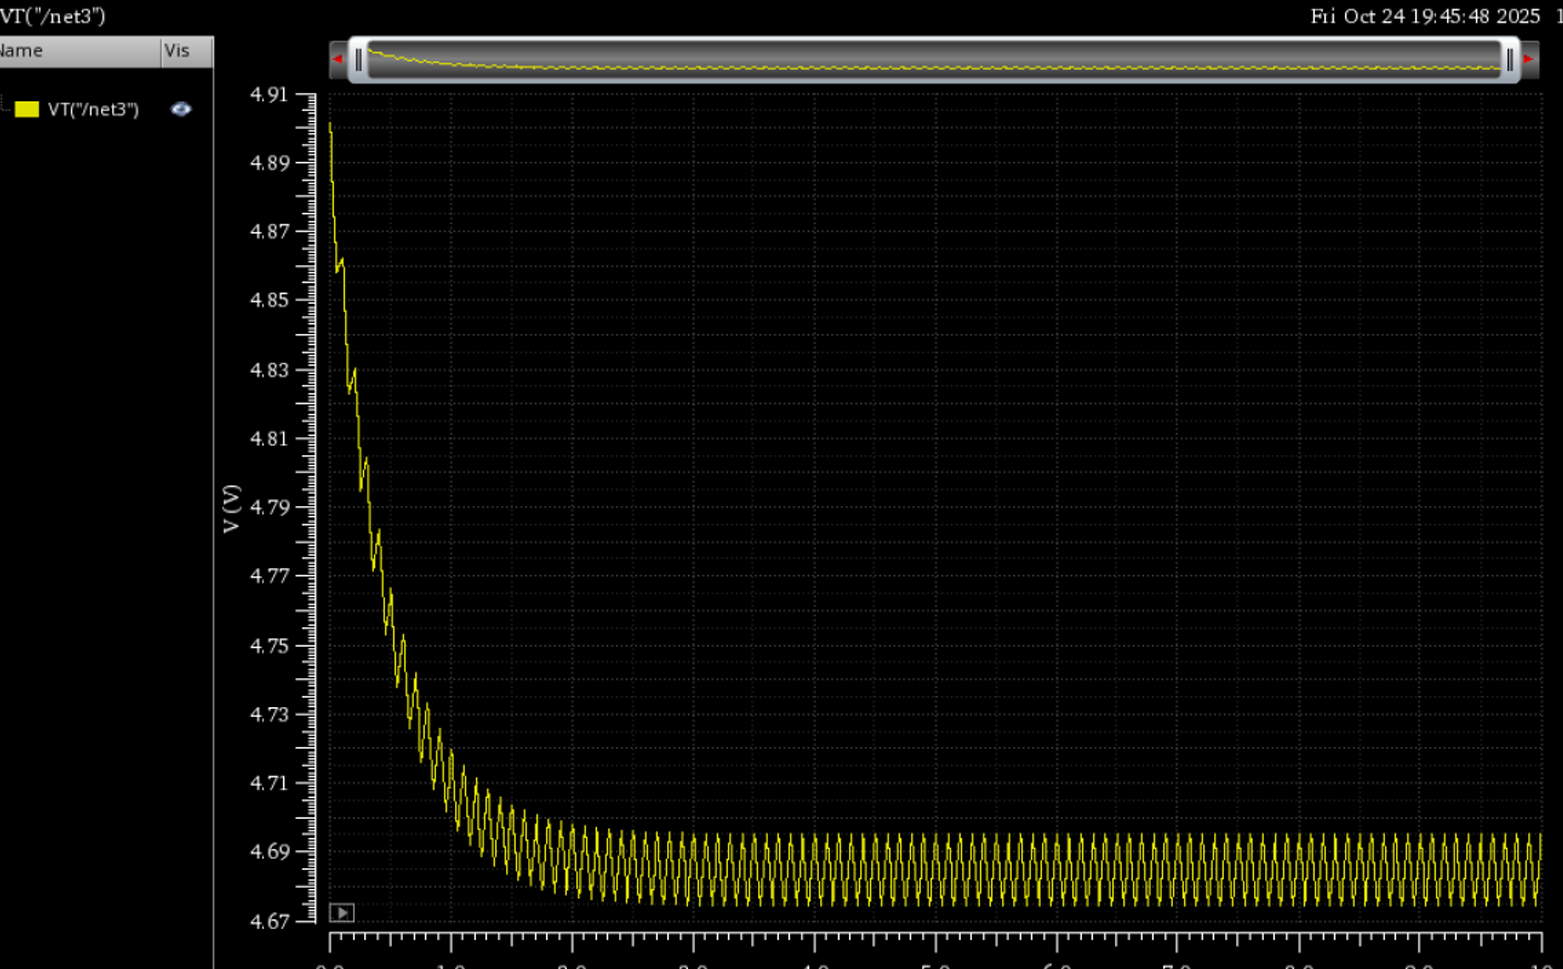
\includegraphics[width=0.8\textwidth]{chapters/figure/A20/仅A处电容.png}
\caption{A位置电容结果}
\label{A位置电容结果}
\end{figure}

\tt{可以看出A位置无电容振幅大约0.4V,加入电容后约0.04V，可以满足设计要求，输出电压纹波较小}

\subsection{B位置的电容:}

\begin{figure}[!ht]
\centering
\resizebox{1\textwidth}{!}{%
\begin{circuitikz}
\tikzstyle{every node}=[font=\normalsize]
\draw (3,11.25) to[american voltage source,l={ \normalsize 5V}] (3,8.5);
\draw (3,11.25) to[european resistor,l={ \normalsize $R_{1}=10\Omega$}] (6,11.25);
\draw (7.25,11.25) to[european resistor,l={ \normalsize $R_{2}=10\Omega$}] (10,11.25);
\draw (7.25,9.5) to[european resistor,l={ \normalsize $R_{a}=1k\Omega$}] (7.25,7);
\draw (11.5,9.25) to[european resistor,l={ \normalsize $R_{d1}=990\Omega$}] (11.5,7);
\draw (13.75,9.25) to[european resistor,l={ \normalsize $R_{d2}=90\Omega$}] (13.75,7);
\draw (6,11.25) to[short] (8,11.25);
\draw (9.75,11.25) to[short] (12.75,11.25);
\draw (12.75,11.25) to[short] (12.75,10);
\draw (12.75,10) to[short] (12,9.25);
\draw (3,8.5) to[short] (3,7);
\draw (3,7) to[short] (13.5,7);
\node [font=\normalsize] at (14.25,10.5) {开关频率10MHz};
\draw (7.25,11.25) to[short] (7.25,9.25);
\draw (3,7) to (3,6.25) node[ground]{};
\node [font=\normalsize] at (6.25,11.75) {A};
\node [font=\normalsize] at (11.75,11.75) {B};
\draw (9.5,9) to[C,l={ \normalsize 26.6nF}] (9.5,7);
\draw (13,7) to[short] (13.75,7);
\draw (9.5,9) to[short] (9.5,11.25);
\end{circuitikz}
}%
\caption{B位置存在26.6nF电容的电路图}
\label{fig:my_label}
\end{figure}

\tt{将电容从A位置移到B位置，仿真结果如下}

\begin{figure}[H]
\centering
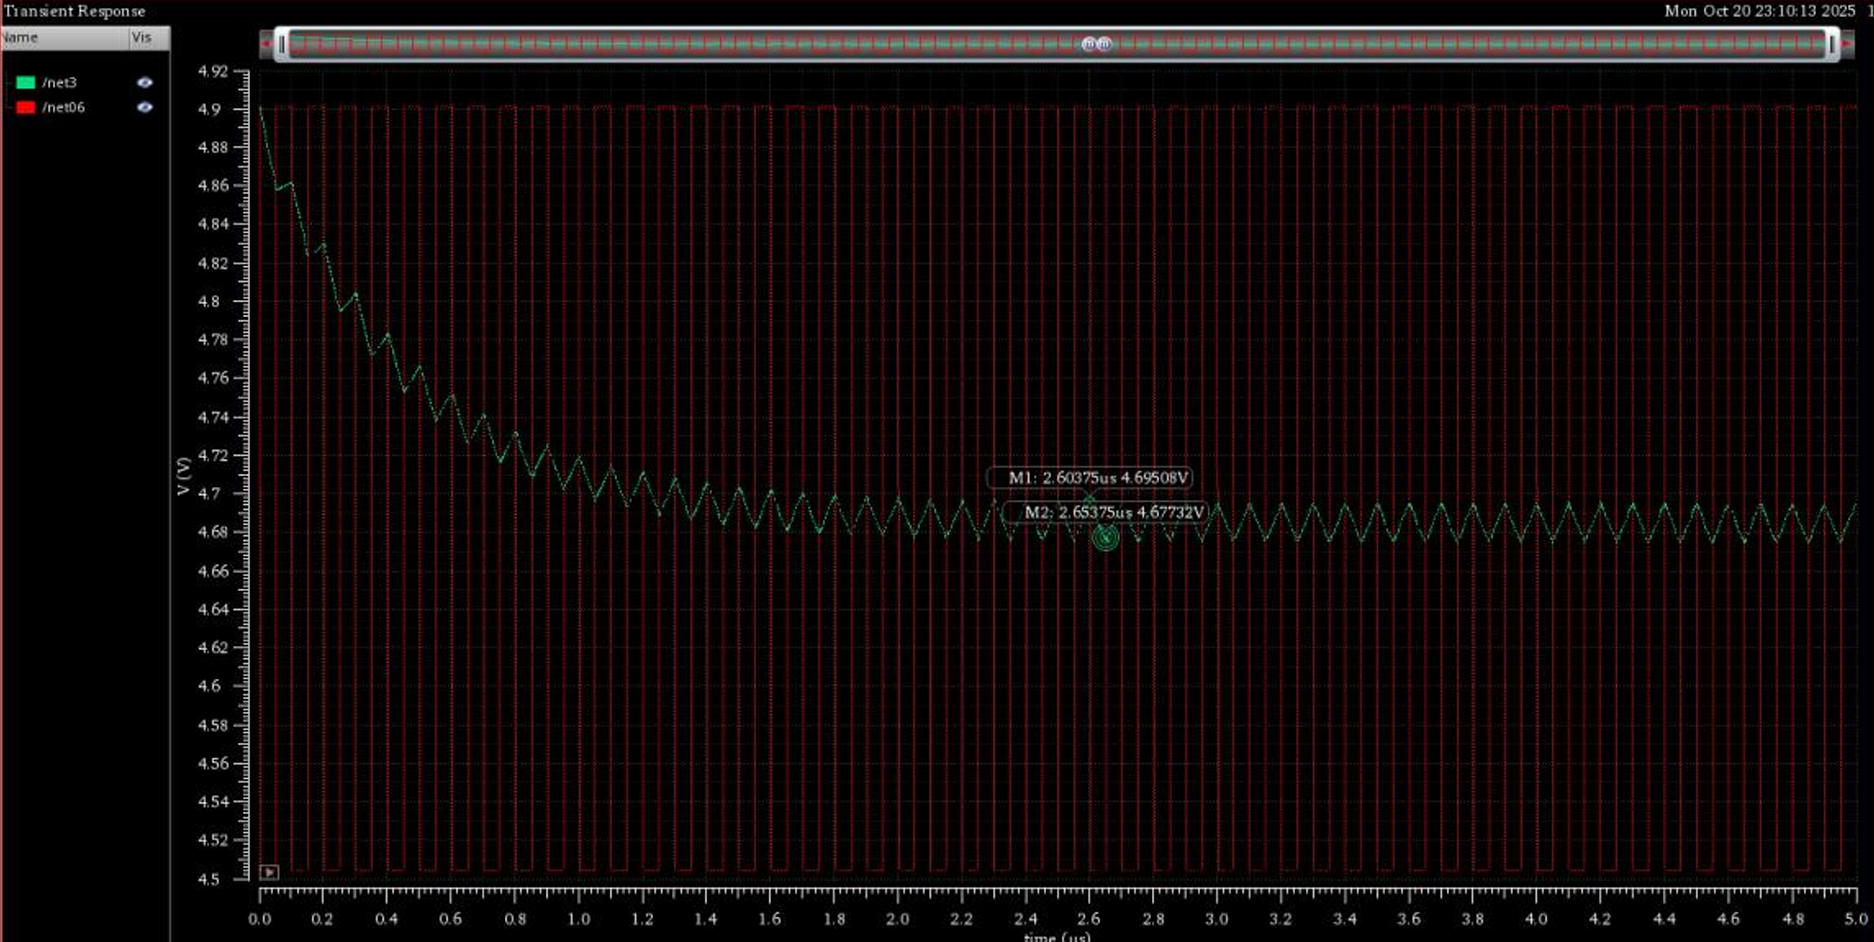
\includegraphics[width=0.8\textwidth]{chapters/figure/A20/B处电容.png}
\caption{B位置电容结果}
\label{B位置电容结果}
\end{figure}

\tt{可以看出B位置无电容振幅大约0.4V,加入电容后约0.018V，可以满足设计要求，且效果更好}

\subsection{AB都有电容}

\begin{figure}[!ht]
\centering
\resizebox{1\textwidth}{!}{%
\begin{circuitikz}
\tikzstyle{every node}=[font=\normalsize]
\draw (3,11.25) to[american voltage source,l={ \normalsize 5V}] (3,8.5);
\draw (3,11.25) to[european resistor,l={ \normalsize $R_{1}=10\Omega$}] (6,11.25);
\draw (7.25,11.25) to[european resistor,l={ \normalsize $R_{2}=10\Omega$}] (10,11.25);
\draw (7.25,9.5) to[european resistor,l={ \normalsize $R_{a}=1k\Omega$}] (7.25,7);
\draw (11.5,9.25) to[european resistor,l={ \normalsize $R_{d1}=990\Omega$}] (11.5,7);
\draw (13.75,9.25) to[european resistor,l={ \normalsize $R_{d2}=90\Omega$}] (13.75,7);
\draw (6,11.25) to[short] (8,11.25);
\draw (9.75,11.25) to[short] (12.75,11.25);
\draw (12.75,11.25) to[short] (12.75,10);
\draw (12.75,10) to[short] (12,9.25);
\draw (3,8.5) to[short] (3,7);
\draw (3,7) to[short] (13.5,7);
\node [font=\normalsize] at (14.25,10.5) {开关频率10MHz};
\draw (7.25,11.25) to[short] (7.25,9.25);
\draw (3,7) to (3,6.25) node[ground]{};
\node [font=\normalsize] at (6.25,11.75) {A};
\node [font=\normalsize] at (11.75,11.75) {B};
\draw (9.5,9) to[C,l={ \normalsize 13.3nF}] (9.5,7);
\draw (13,7) to[short] (13.75,7);
\draw (9.5,9) to[short] (9.5,11.25);
\draw (5.25,9.25) to[C,l={ \normalsize 13.3nF}] (5.25,7);
\draw (5.25,9) to[short] (5.25,11.25);
\end{circuitikz}
}%
\caption{A、B位置都有13.3nF电容的电路图}
\label{fig:my_label}
\end{figure}

\begin{figure}[H]
\centering
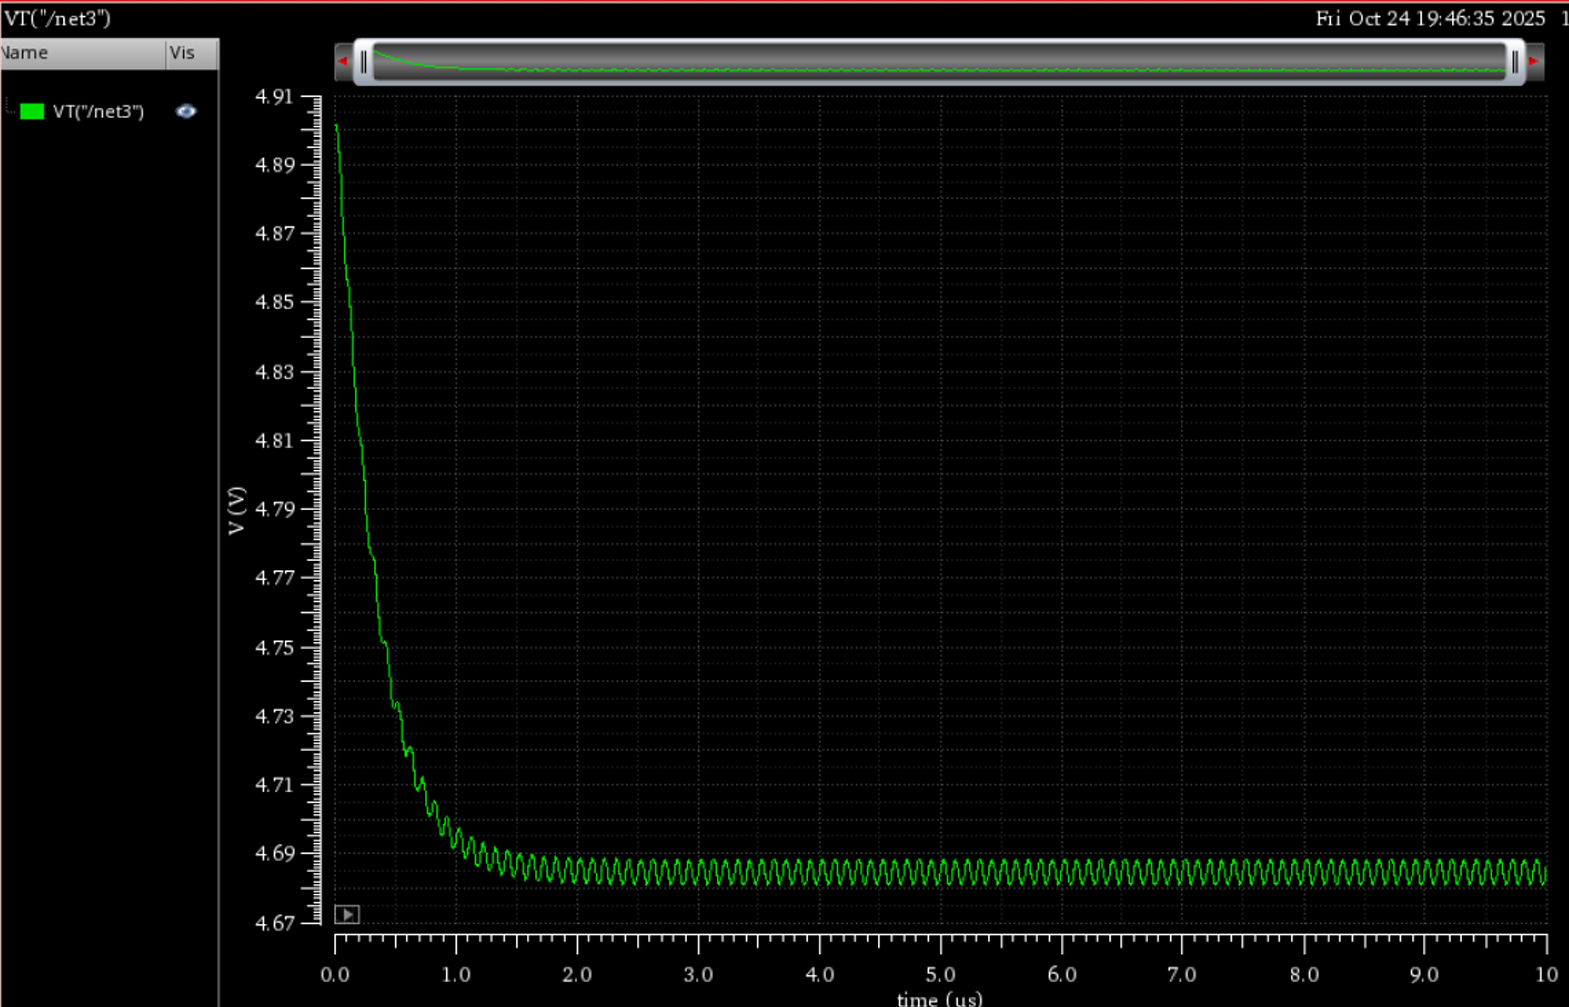
\includegraphics[width=0.8\textwidth]{chapters/figure/A20/AB处电容.png}
\caption{A、B位置都有13.3nF电容结果}
\label{AB位置电容结果}
\end{figure}

\tt{可以看出加入电容后约0.01V，可以满足设计要求，且效果更好}

\subsection{AB及互导电阻中间都有电容}

\begin{figure}[!ht]
\centering
\resizebox{1\textwidth}{!}{%
\begin{circuitikz}
\tikzstyle{every node}=[font=\normalsize]
\draw (0.75,11.25) to[american voltage source,l={ \normalsize 5V}] (0.75,8.5);
\draw (3.5,11.25) to[european resistor,l={ \normalsize $5\Omega$}] (5.25,11.25);
\draw (7.25,11.25) to[european resistor,l={ \normalsize $5\Omega$}] (9.25,11.25);
\draw (7.25,7) to[european resistor,l={ \normalsize $R_{a}=1k\Omega$}] (7.25,9.5);
\draw (13.5,9.25) to[european resistor,l={ \normalsize $R_{d1}=990\Omega$}] (13.5,7);
\draw (15.75,9.25) to[european resistor,l={ \normalsize $R_{d2}=90\Omega$}] (15.75,7);
\draw (6,11.25) to[short] (7.25,11.25);
\draw (11.25,11.25) to[short] (14.75,11.25);
\draw (14.75,11.25) to[short] (14.75,10);
\draw (14.75,10) to[short] (14,9.25);
\draw (0.75,8.75) to[short] (0.75,7.25);
\draw (0.75,7) to[short] (15.75,7);
\node [font=\normalsize] at (16.5,10.5) {开关频率10MHz};
\draw (7.25,11.25) to[short] (7.25,9.25);
\draw (0.75,7.25) to (0.75,6.5) node[ground]{};
\node [font=\normalsize] at (6.25,11.75) {A};
\node [font=\normalsize] at (11.75,11.75) {B};
\draw (12,7) to[C,l={ \normalsize 8.9nF}] (12,9);
\draw (13,7) to[short] (13.75,7);
\draw (12,9) to[short] (12,11.25);
\draw (5.25,7) to[C,l={ \normalsize 8.9nF}] (5.25,9.25);
\draw (5.25,9) to[short] (5.25,11.25);
\draw (5.25,11.25) to[short] (6,11.25);
\draw (9.75,11.25) to[european resistor,l={ \normalsize $5\Omega$}] (11.25,11.25);
\draw (0.75,11.25) to[european resistor,l={ \normalsize 5$\Omega$}] (2.5,11.25);
\draw (9.5,7) to[C,l={ \normalsize 8.9nF}] (9.5,9);
\draw (9.25,11.25) to[short] (10,11.25);
\draw (9.5,9) to[short] (9.5,11.25);
\draw (2.25,11.25) to[short] (3.75,11.25);
\end{circuitikz}
}%

\label{fig:my_label}
\end{figure}

\begin{figure}[H]
\centering
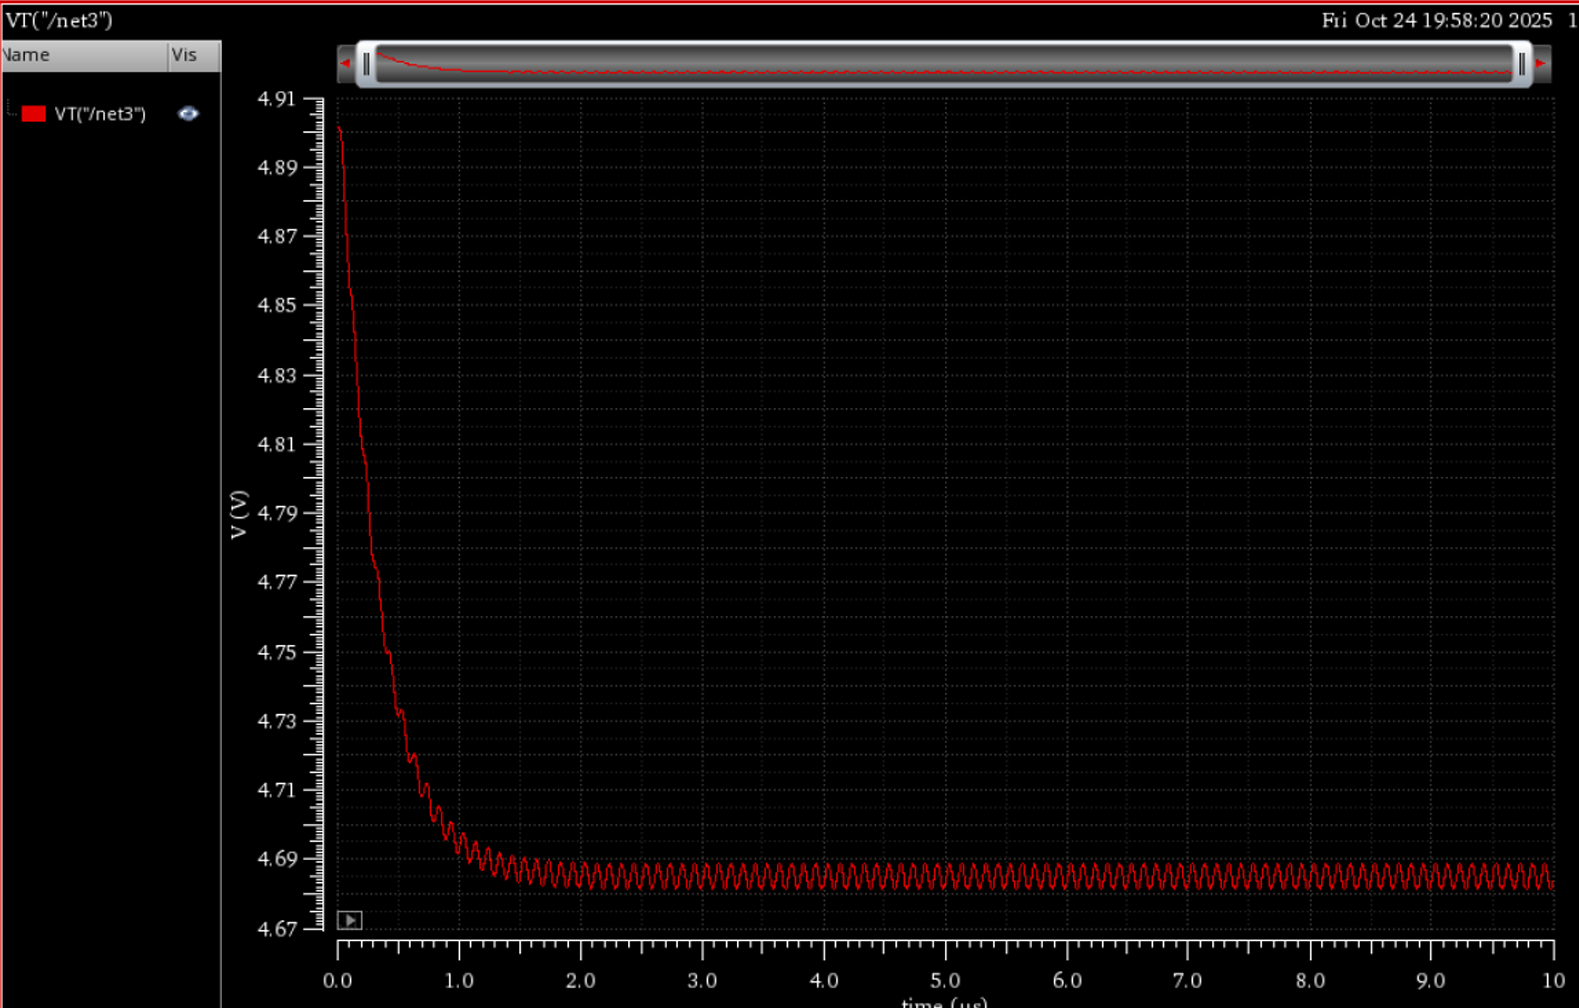
\includegraphics[width=0.8\textwidth]{chapters/figure/A20/AB及互导电阻中间都有电容.png}
\caption{A、B位置及互导电阻中间都有8.9nF电容结果}
\label{AB及互导电阻中间都有电容结果}
\end{figure}

\tt{可以看出加入电容后约0.01V，可以满足设计要求，差别不大}

\subsection{AB及互导、互阻电阻中间都有电容}

\begin{figure}[!ht]
\centering
\resizebox{1\textwidth}{!}{%
\begin{circuitikz}
\tikzstyle{every node}=[font=\normalsize]
\draw (0.75,11.25) to[american voltage source,l={ \normalsize 5V}] (0.75,8.5);
\draw (3.5,11.25) to[european resistor,l={ \normalsize $5\Omega$}] (5.25,11.25);
\draw (7.25,11.25) to[european resistor,l={ \normalsize $5\Omega$}] (9.25,11.25);
\draw (7.25,7) to[european resistor,l={ \normalsize $R_{a}=1k\Omega$}] (7.25,9.5);
\draw (13.5,9.25) to[european resistor,l={ \normalsize $R_{d1}=990\Omega$}] (13.5,7);
\draw (15.75,9.25) to[european resistor,l={ \normalsize $R_{d2}=90\Omega$}] (15.75,7);
\draw (6,11.25) to[short] (7.25,11.25);
\draw (11.25,11.25) to[short] (14.75,11.25);
\draw (14.75,11.25) to[short] (14.75,10);
\draw (14.75,10) to[short] (14,9.25);
\draw (0.75,8.75) to[short] (0.75,7.25);
\draw (0.75,7) to[short] (15.75,7);
\node [font=\normalsize] at (16.5,10.5) {开关频率10MHz};
\draw (7.25,11.25) to[short] (7.25,9.25);
\draw (0.75,7.25) to (0.75,6.5) node[ground]{};
\node [font=\normalsize] at (6.25,11.75) {A};
\node [font=\normalsize] at (11.75,11.75) {B};
\draw (12,7) to[C,l={ \normalsize 6.6nF}] (12,9);
\draw (13,7) to[short] (13.75,7);
\draw (12,9) to[short] (12,11.25);
\draw (5.25,7) to[C,l={ \normalsize 6.6nF}] (5.25,9.25);
\draw (5.25,9) to[short] (5.25,11.25);
\draw (5.25,11.25) to[short] (6,11.25);
\draw (9.75,11.25) to[european resistor,l={ \normalsize $5\Omega$}] (11.25,11.25);
\draw (0.75,11.25) to[european resistor,l={ \normalsize 5$\Omega$}] (2.5,11.25);
\draw (9.5,7) to[C,l={ \normalsize 6.6nF}] (9.5,9);
\draw (9.25,11.25) to[short] (10,11.25);
\draw (9.5,9) to[short] (9.5,11.25);
\draw (2.25,11.25) to[short] (3.75,11.25);
\draw (2.75,7) to[C,l={ \normalsize 6.6nF}] (2.75,9.25);
\draw (2.75,11.25) to[short] (2.75,8.75);
\end{circuitikz}
}%
\caption{A、B位置及互导、互阻电阻中间都有6.6nF电容的电路图}
\label{fig:my_label}
\end{figure}

\begin{figure}[H]
\centering
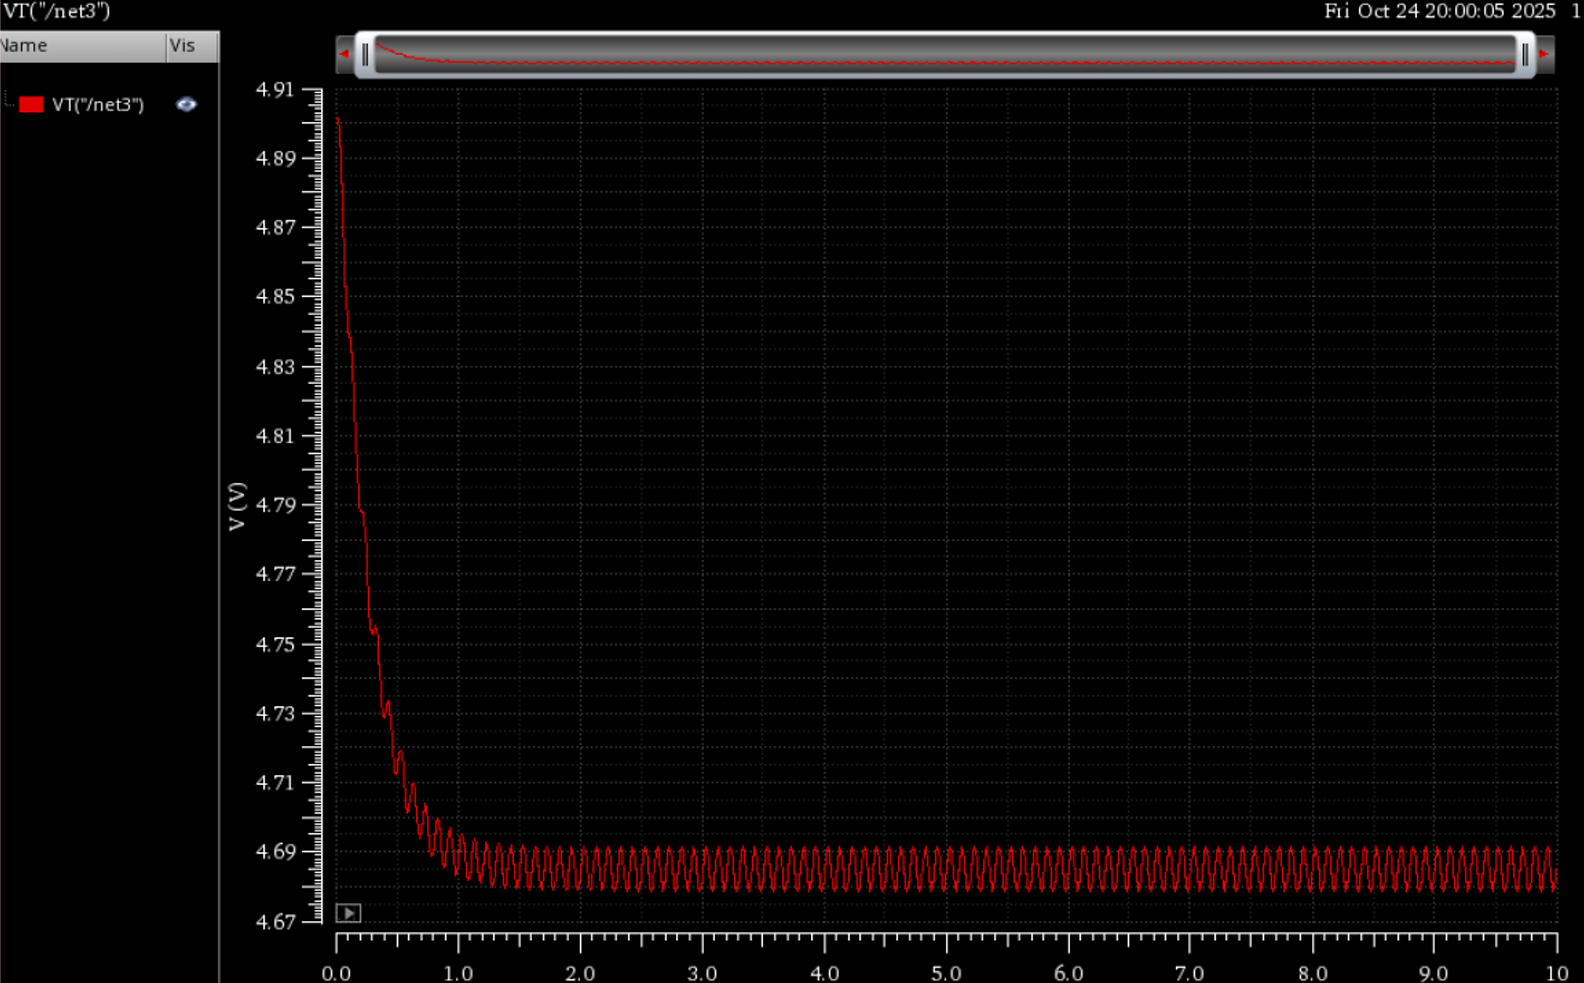
\includegraphics[width=0.8\textwidth]{chapters/figure/A20/AB及互导、互阻电阻中间都有电容.png}
\caption{A、B位置及互导、互阻电阻中间都有6.6nF电容结果}
\label{AB及互导、互阻电阻中间都有电容结果}
\end{figure}

\tt{可以看出加入电容后约0.01V，可以满足设计要求，差别不大}

\subsection{总结:}
\tt{功能电路的去耦电容应该置于什么位置最好？}

\tt{去耦电容应该置于离负载更近的位置，效果更好}

\subsection{继续研究：模拟电路还是数字电路离电源更近了好？}

\tt{模拟电路离电源更近了好，因为模拟电路对电压纹波更敏感，去耦电容放在离模拟电路更近的位置可以更有效地降低电压纹波，保证模拟电路的稳定性和性能}

\begin{figure}[H]
\centering
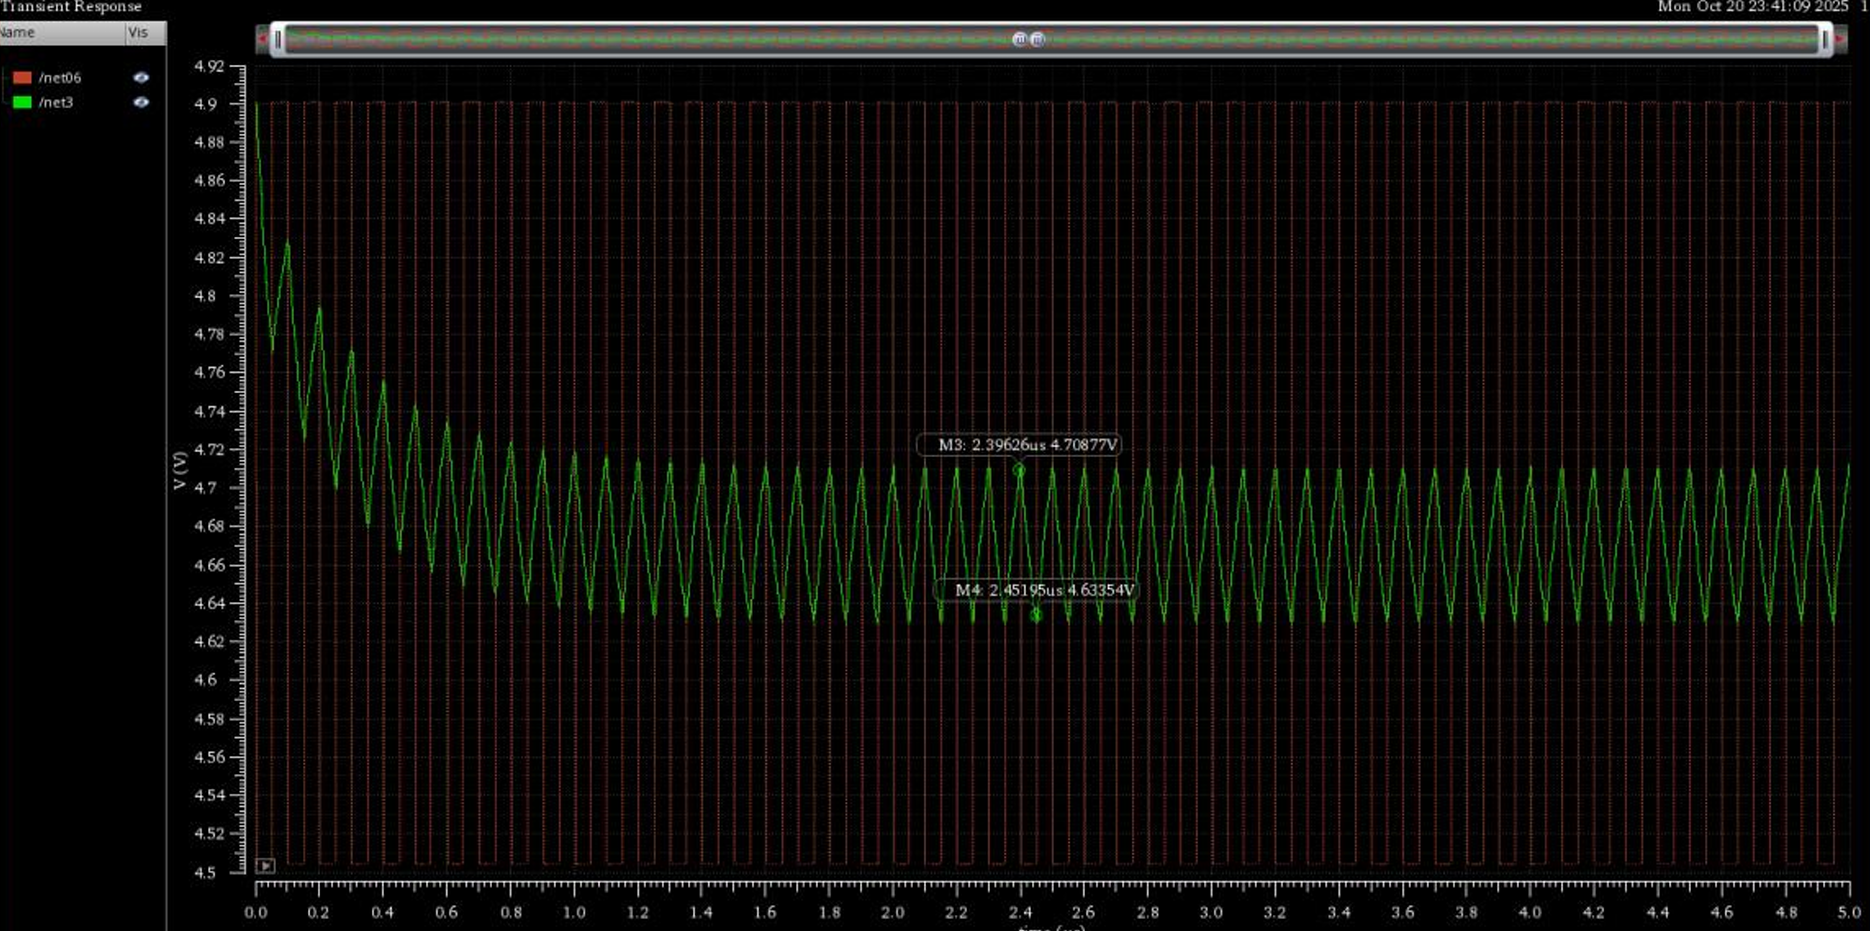
\includegraphics[width=0.8\textwidth]{chapters/figure/A20/互换.png}
\caption{显然互换后效果更差了}
\label{AB及互导、互阻电阻中间都有电容结果}
\end{figure}